\section{Experiments}\label{sec:experiment}



We experimentally evaluated our approach. In the following of this section, we first present the testing infrastructure adopted in our experiments,
then we discuss the experimental settings, and
finally we discuss the performance of our heuristic algorithm.

\subsection{Testing Infrastructure and Settings}

We designed and developed a Python-based testing infrastructure that implements the emulation of service execution, comparison and composition.
The emulator implements the sliding window heuristic for the generation of the best service composition, to asses its effectiveness and efficiency, in terms of execution time and approximation of the optimal solution.
To better evaluate the performance of the heuristic algorithm, we also implemented the optimal solution, which is obtained by executing all possible combinations of services for each node.
The emulator simplify the execution of the service composition by removing the service selection phase, which is not relevant for the purpose of the experiment.
All our experiments have been run on a workstation equipped with a 2.40GHz i5-8279U CPU with 16GB RAM and a 512GB SSD.

\subsection{ Evaluation}
% \subsection{performance}
% \begin{itemize}
%   \item Finestra scorrevole da 1 a N=Nodi
%   \item Servizi 5 a 20 passo 5 + 50??
%   \item
% \end{itemize}
% \subsection{Metriche/Euristiche}

The procedure was repeated by varying only one service at a time and executing the entire pipeline.
The experiments were primarily evaluated along three dimensions:

(i) Evaluation of the exhaustive execution time of all combinations by incrementing the number of services and nodes periodically:
This experiment aimed to comprehend how execution time fluctuates with increasing numbers of nodes and services.
The number of nodes was varied from 1 to 6, while the number of services was varied from 2 to 20, with a step of 1.
The execution has been stopped at the first combination that reported an execution time greater than 10k seconds.
The observed trend aligns with expectations, exhibiting exponential growth in execution times as the number of nodes increases.

Refer to Table X for a graphical representation.

(ii) Evaluation of execution time with the introduction of heuristics:
The heuristics, as defined in the relevant section, were incorporated,
and the entire pipeline was rerun with variations in the number of nodes,
services, and the size of the sliding window.

Notably, a window of size 1 corresponds to a greedy algorithm execution,
while a window of size n, where n is the number of nodes, is analogous to exhaustive execution.

(iii) Comparison of the optimal versus heuristics:
The optimal combination, characterized by the least data loss in the execution of the entire pipeline,
was determined by computing the minimum coefficient of variation for each combination.
The computation of the optimum necessitates exhaustive execution, involving all possible combinations of candidate services at each node.
Heuristics reduce execution time by approximating this selection through the use of a sliding window and generating all combinations within the window.
The objective of this final experiment is to assess the disparity between the optimum obtained with the sliding window and that obtained through exhaustive execution.

To introduce a level of interdependence among services,
matrices containing the degrees of dependence of each service with the next were employed.
It is important to note that different definitions of the optimum may yield slightly different results.

\begin{figure}
  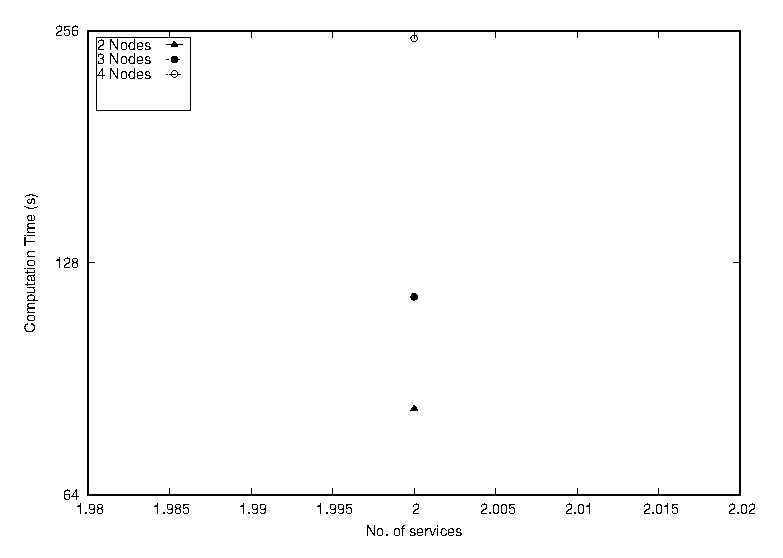
\includegraphics[width=0.95\columnwidth]{graphs/exhaustive_performance.eps}
  \caption{Preliminary performance evaluation.}
  \label{fig:perf_exhaustive}
\end{figure}
\begin{figure*}
  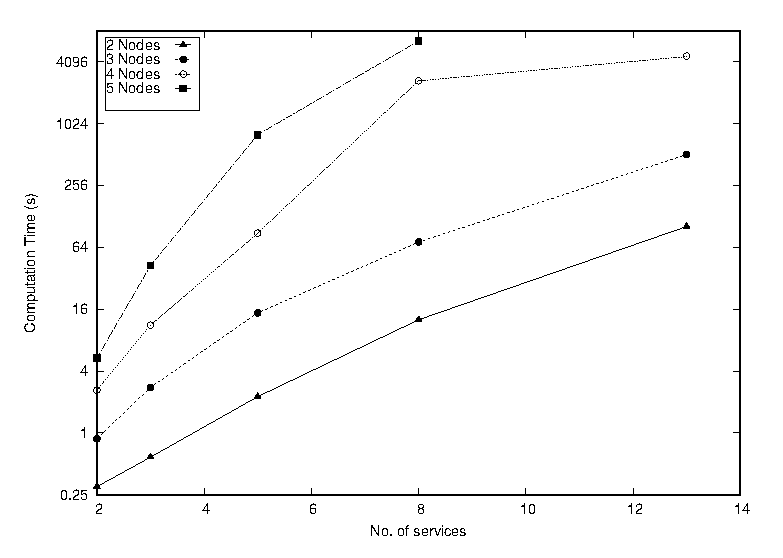
\includegraphics[width=0.95\textwidth]{graphs/window_performance.eps}
  \caption{Preliminary performance evaluation.}
  \label{fig:perf_window}
\end{figure*}


\section{Pipeline Instance}\label{sec:instance}
% \subsection{Instance}
% \hl{ANCHE QUA COME PER IL TEMPLATE PROVEREI A ESSERE UN POCO PIU' FORMALE. GUARDA IL PAPER CHE TI HO PASSATO.}
We define a pipeline instantiation technique as a function that takes as input a \pipelineTemplate \tChartFunction and a set $S^c$ of candidate services, one for each vertex \vi{i}$\in$\V, and returns as output a \pipelineInstance \iChartFunction.
%We recall that candidate services $S^c_i$ are candidate services satisfying data protection annotations \myLambda(\vi{i}), for each \vi{i}$\in$$\V_S$.
In \iChartFunction, every invocations \vii{i}$\in$$V'_S$ contains a service instance, and every branching $v\in\Vplus\bigcup\Vtimes$ in the template is maintained as is. We formally define our \pipelineInstance as follows.

    \begin{definition}[Pipeline Instance]\label{def:instance}
      Let \tChartFunction be a pipeline template, a pipeline Instance $\iChartFunction$ is a directed acyclic graph where:
      \begin{enumerate*}[label=\textit{\roman*})]
        \item $s_r$$=$$s'_r$;
        \item for each vertex $\vi{}\in\V_{\timesOperator}\cup\V_{\plusOperator}$ it exists a corresponding vertex $\vii{}\in\Vp_{\timesOperator}\cup\Vp_{\plusOperator}$;
        \item for each $\vi{i}$$\in$$\V_S$ annotated with policy \P{i} it exists a corresponding \vii{i}$\in$$\Vp_S$ instantiated with a service instance \sii{i};
      \end{enumerate*}
      and such that the following conditions hold:
      \begin{enumerate}[label=\arabic*)]
        \item $s'_i$ satisfies data protection annotation \myLambda(\vi{i}) in \tChartFunction;
        \item $s'_i$ satisfies functional annotation \myGamma(\vi{i}) in \tChartFunction.
      \end{enumerate}
    \end{definition}

    Condition 1 is needed to preserve the process functionality, as it simply states that each service \sii{i} must satisfy the functional requirements \F{i} of the corresponding vertex \vi{i} in the \pipelineTemplate.
    Condition 2 states that each service \sii{i} must satisfy the policy requirements \P{i} of the corresponding vertex \vi{i} in the \pipelineTemplate.
    We recall that Condition 1 is satisfied for all candidate services (see Section~\ref{sec:funcannotation}) and therefore concentrate on Condition 2 in the following.

    The \pipelineInstance  is generated by traversing the \pipelineTemplate with a breadth-first search algorithm, starting from the root vertex \vi{r}.
    Then, for each vertex $v\in\Vplus\bigcup\Vtimes$ in the pipeline template, the corresponding vertex $v'\in\Vpplus\bigcup\Vptimes$ is generated.
    Finally, for each vertex \vi{i}$\in$$\V_S$, a two-step selection approach is applied as follows.
  \begin{itemize}

    \item \textit{Filtering Algorithm} -- As already discussed in Section~\ref{sec:templatedefinition}, filtering algorithm retrieves a set of candidate services $S^c$ and match them one-by-one against data protection requirements \myLambda(\vi{i}). In particular, the profile of each candidate service \si{j} is matched against policies $p_k$$\in$\P{i} corresponding to \myLambda(\vi{i}). Filtering algorithm returns as output the set of compatible services that match the policy.

                Formally, let us consider a set $S^c$ of candidate services \si{j}, each one having a profile as a set of attributes in the form (\emph{name}, \emph{value}). The filtering algorithm is executed for each \si{j}; it is successful if \si{j}'s profile satisfies at least one policy $p_k$$\in$\P{i}; otherwise, \si{j} is discarded and not considered for selection. The filtering algorithm finally returns a subset $S'\subseteq S^c$ of compatible services, among which the service instance is selected.

    \item \textit{Comparison Algorithm} -- Upon retrieving a set $S'$ of compatible services \si{j}, it produces a ranking of these services according to some metrics that evaluates the quality loss introduced by each service when integrated in the pipeline instance. More details about the metrics are provided in Section \ref{sec:metrics}.
          %Formally, compatible services \si{j}$\in$S' are ranked on the basis of a scoring function.
          The best service $s'_i$ is then selected and integrated in $\vii{i}\in \Vp$. There are many ways of choosing relevant metrics, we present those used in this article in Section \ref{sec:metrics}.
  \end{itemize}

  When all vertices $\vi{i}\in V$ have been visited, G' contains a service instance $s'_i$ for each \vii{i}$\in$\Vp, and the \pipelineInstance is complete. We note that each vertex \vii{i} is annotated with policies $p_k$$\in$\P{i} according to \myLambda. When pipeline instance is triggered, before any services can be executed, policies in \P{i} are evaluated and enforced. In case policy evaluation returns \emph{true}, data transformation \TP$\in$\P{i} is applied, otherwise a default transformation that removes all data is applied.

\usetikzlibrary{positioning}
\usetikzlibrary{backgrounds}



\begin{figure}[ht!]
  \centering
  \newcommand{\function}{$\instanceChartAnnotation{}$}
  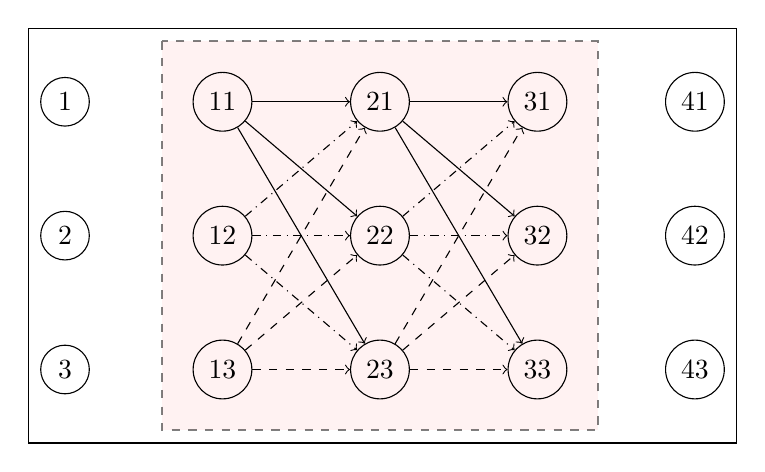
\begin{tikzpicture}[framed]
    \node[draw, circle] (s41) at (1,1.7) {$\sii{1}$};
    \node[draw, circle] (s42) at (1,0) {$\sii{2}$};
    \node[draw, circle] (s43) at (1,-1.7) {$\sii{3}$};

    \node[draw, circle] (s1) at (3,1.7) {$\sii{11}$};
    \node[draw, circle] (s2) at (3,0) {$\sii{12}$};
    \node[draw, circle] (s3) at (3,-1.7) {$\sii{13}$};

    \node[draw, circle] (s11) at (5,1.7) {$\sii{21}$};
    \node[draw, circle] (s12) at (5,0) {$\sii{22}$};
    \node[draw, circle] (s13) at (5,-1.7) {$\sii{23}$};

    \node[draw, circle] (s21) at (7,1.7) {$\sii{31}$};
    \node[draw, circle] (s22) at (7,0) {$\sii{32}$};
    \node[draw, circle] (s23) at (7,-1.7) {$\sii{33}$};

    \node[draw, circle] (s31) at (9,1.7) {$\sii{41}$};
    \node[draw, circle] (s32) at (9,0) {$\sii{42}$};
    \node[draw, circle] (s33) at (9,-1.7) {$\sii{43}$};


    % \draw[->] (node2) -- (node3);
    \draw[->] (s1) -- (s11);
    \draw[->] (s1) -- (s12);
    \draw[->] (s1) -- (s13);

    \draw[->,dashdotted] (s2) -- (s11);
    \draw[->,dashdotted] (s2) -- (s12);
    \draw[->,dashdotted] (s2) -- (s13);

    \draw[->,dashed] (s3) -- (s11);
    \draw[->,dashed] (s3) -- (s12);
    \draw[->,dashed] (s3) -- (s13);


    \draw[->] (s11) -- (s21);
    \draw[->] (s11) -- (s22);
    \draw[->] (s11) -- (s23);

    \draw[->,dashdotted] (s12) -- (s21);
    \draw[->,dashdotted] (s12) -- (s22);
    \draw[->,dashdotted] (s12) -- (s23);

    \draw[->,dashed] (s13) -- (s21);
    \draw[->,dashed] (s13) -- (s22);
    \draw[->,dashed] (s13) -- (s23);


    \begin{scope}[on background layer]
      \draw[thick, dashed, fill=red!10, opacity=0.5]
      ([shift={(-0.5,0.5)}]s1.north west) rectangle ([shift={(0.5,-0.5)}]s23.south east);

    \end{scope}


  \end{tikzpicture}
  \caption{Service composition instance}
  \label{fig:service_composition_instance}
\end{figure}
